\documentclass[a4paper,10pt]{article}

\usepackage[activeacute]{babel}
\usepackage[utf8]{inputenc}
\usepackage{bookman}
\usepackage{color}
\usepackage{graphicx}
\usepackage{anysize}
\usepackage{multicol}
\usepackage[pdftex=true,colorlinks=true,linkcolor=black,urlcolor=blue]{hyperref}

\marginsize{1.5cm}{1.5cm}{1.5cm}{1.5cm}
\newcommand{\HRule}{\rule{\linewidth}{0.5mm}}

\date{}

\pagenumbering{arabic}
\setcounter{page}{1}

\begin{document}

% ===================================== MEMBRETE ===================================== %
\begin{center}
  \textsc {
    Universidad Simón Bolívar \\[0cm]
    Departamento de Computaci\'on y Tecnolog\'ia de la Informaci\'on \\[0cm]
    CI5438 - Inteligencia Artificial I \\[0cm]
    Trimestre Abril - Julio 2021 \\[0cm]
    Prof. Carlos Infante \\[0cm]
    Amin Arriaga 16-10072, David Segura XX-XXXXX, Wilfredo Graterol XX-XXXXX
  }
  \HRule \\[0.4cm]
  {\Large \textbf{B\'usqueda Informada: A* vs IDA*}} \\[0.4cm]
  \textsc{
    \today
  }
  \HRule
\end{center}

\section{Introducci\'on}

\section{Estructura del Repositorio}
  El repositorio presenta la siguiente estructura de archivos:

  \begin{verbatim}
    proyecto-1-ci5437/
    |__ benchmarks/...
    |__ bin/...
    |__ generators
    |   |__ HanoisTowersGenerator.py
    |   |__ SlidingTileGenerator.py
    |   |__ TopSpinGenerator.py
    |__ informe.pdf -> src/L_informe/informe.pdf
    |__ Makefile
    |__ papers/...
    |__ pdbs/...
    |__ psvn/...
    |__ puzzles/...
    |__ README.md
    |__ resources/...
    |__ src
        |__ head.hpp
        |__ heuristics.cpp
        |__ heuristics.hpp
        |__ InformedSearchs.cpp
        |__ InformedSearchs.hpp
        |__ L_informe/...
        |__ main.cpp
        |__ Node.cpp
        |__ Node.hpp
        |__ NodesPriorityQueue.cpp
        |__ NodesPriorityQueue.hpp
        |__ PriorityQueue.hpp
  \end{verbatim}

  donde 

  \begin{itemize}
    \item \verb|bin/| contiene los archivos binarios que resuelven alg\'un puzzle.
    Los archivos en este directorio tienen el formato \verb|P.out| donde \verb|P|
    es el nombre de alg\'un puzzle. Estos archivos no son agregados al repositorio.

    \item \verb|generators/| contiene los generadores de archivos \verb|.psvn|.
    Los que se encuentran actualmente son:
    \begin{itemize}
      \item \verb|generators/HanoisTowersGenerator.py| tal que al ejecutarse con 
      \verb|P > 2| y \verb|D > 1|, imprime un PSVN el puzzle de las Torres 
      de Hanoi con \verb|P| astas y \verb|D| discos.

      \item \verb|generators/SlidingTileGenerator.py| tal que al ejecutarse con 
      \verb|M > 0| y \verb|N > 0|, imprime un PSVN el puzzle de Sliding 
      Tiles con dimensi\'on \verb|M x N|.

      \item \verb|generators/TopSpinGenerator.py| tal que al ejecutarse con 
      \verb|K > 1| y \verb|N > K|, imprime un PSVN el puzzle Top Spin con 
      \verb|N| tokens y un 'turntable' de longitud \verb|K|.
    \end{itemize}

    \item \verb|pdbs/| contiene los archivos necesarios para generar PDBs para los 
    distintos puzzles a estudiar. Revise el archivo \verb|pdbs/README.md| para m\'as
    informaci\'on.

    \item \verb|psvn/| contiene el c\'odigo fuente para compilar la API de PSVN.
    
    \item \verb|puzzles/| contiene archivos \verb|.psvn|.

    \item \verb|src/| contiene el c\'odigo fuente principal para compilar y ejecutar 
    los distintos algoritmos de b\'usqueda informada que estudiaremos en este proyecto.
    Daremos una brvee explicaci\'on de cada archivo:
    \begin{itemize}
      \item \verb|src/Node.*| tiene la implementaci\'on de nodo que hemos usado durante 
      las clases. Tambi\'en almacena la profundidad del camino parcial hasta ese nodo.

      \item \verb|src/PriorityQueue.hpp| tiene la implementaci\'on de una cola de 
      prioridad gen\'erica. Permite definir el tipo de dato que servir\'a para realizar 
      las comparaciones, el tipo de los elementos que almacenar\'a y la funci\'on de 
      comparaci\'on. No se separ\'o en archivos \verb|.cpp| y \verb|.hpp| debido a los 
      problemas de C++ con los templates.

      \item \verb|src/NodesPriorityQueue.*| tiene otra implementaci\'on de una cola de 
      prioridad pero basada en nodos, y que adem\'as de los m\'etodos 
      \verb|empty|, \verb|add| y \verb|pop|, tambi\'en tiene los m\'etodos \verb|find|
      que busca un nodo seg\'un el estado que almacena; y \verb|replace_if_less| que,
      dado un nodo, verifica si la cola tiene otro nodo que representa al mismo estado
      que adem\'as tiene un costo parcial superior al nodo par\'ametro, entonces es 
      sustituido por el nodo par\'ametro. Estas 2 funciones en una cola de prioridad 
      com\'un ser\'ian $O(n)$, lo cual no es deseable en las funciones de b\'usqueda.

      \item \verb|src/InformedSearchs.*| tiene las implementaciones de los algoritmos
      de b\'usqueda que se estudian en el proyecto. En particular, se encuentran los 
      siguientes algoritmos:
      \begin{itemize}
        \item A* sobre grafos.
        \item A* sobre \'arboles.
        \item A* con eliminaci\'on tard\'ia de nodos.
        \item IDA* sobre grafos.
        \item IDA* sobre \'arboles.
        \item IDA* con eliminaci\'on parcial de nodos.
      \end{itemize}

      \item \verb|src/heuristics.*| tiene las implementaciones de las distintas 
      he\'uristicas que se usar\'an, principalmente de PDBs.

      \item \verb|src/main.cpp| y \verb|src/head.hpp| el cual, al compilarse y
      ejecutarse, te permite ingresar un estado inicial, as\'i como escoger un
      algoritmo de b\'usqueda y una heur\'istica de los implementados para resolver
      el puzzle. Consulte el archivo \verb|Makefile| para m\'as informaci\'on.
      
      \item \verb|src/L_informe/| contiene los archivos fuentes de latex necesarios 
      para generar este informe.
    \end{itemize}
    
  \end{itemize}

\section{Casos de Prueba}
  \subsection{15 Puzzle}
    Para el \textit{15 Puzzle} usamos como heur\'istica la distancia Manhattan.
    
    \begin{verbatim}
    STATE (EASY):   14 1 9 6 4 8 12 5 7 2 3 B 10 11 13 15
    |           FUNCTION|   TIME (SEC)|  MEMORY (GB)|       NODES/SEC|    SOL-LEN|
    |                 A*|   172.613782|      5.39361|    138210.58622|         45|
    |         A* pruning|     2.627228|      0.04398|     62283.51708|         45|
    |    A* late pruning|     2.593914|      0.04016|     90053.48674|         45|
    |               IDA*|   294.174137|      0.00055|    243362.32182|         45|
    |       IDA* pruning|     1.537629|       0.0129|    410535.96154|         45|
    |  IDA* part pruning|     2.629333|      0.00024|    240086.36411|         45|
    \end{verbatim}        
    
    \begin{verbatim}  
    STATE (MEDIUM): 12 9 B 6 8 3 5 14 2 4 11 7 10 1 15 13                                                                                       
    |           FUNCTION|   TIME (SEC)|  MEMORY (GB)|       NODES/SEC|    SOL-LEN|
    |                 A*|                    TOO MUCH MEMORY                     |
    |         A* pruning|   361.748725|      2.56905|     26938.20137|         50|
    |    A* late pruning|   184.561287|      2.34054|     85301.65917|         50|
    |               IDA*|                     TOO MUCH TIME                      |
    |       IDA* pruning|   243.698492|      0.00148|    413353.29231|         50|
    |  IDA* part pruning|   421.172057|       0.0001|    239603.34577|         50|
    \end{verbatim}

    \begin{verbatim}  
    STATE (HARD):   5 9 13 14 6 3 7 12 10 8 4 B 15 2 11 1                                                                                     
    |           FUNCTION|   TIME (SEC)|  MEMORY (GB)|       NODES/SEC|    SOL-LEN|
    |                 A*|                    TOO MUCH MEMORY                     |  
    |         A* pruning|   633.547779|       4.1973|     25436.99234|         57|
    |    A* late pruning|   305.977159|      3.92621|     77683.54042|         57|
    |               IDA*|                     TOO MUCH TIME                      |
    |       IDA* pruning|   349.547181|      0.00082|    404336.85832|         57|
    |  IDA* part pruning|   591.625852|      0.00195|    238931.14461|         57|
      \end{verbatim}

    \begin{figure*}[h!]
      \centering
      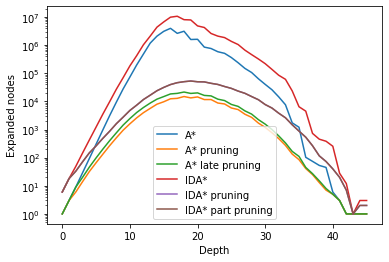
\includegraphics[scale=0.6]{15puzzle_easy.png}
      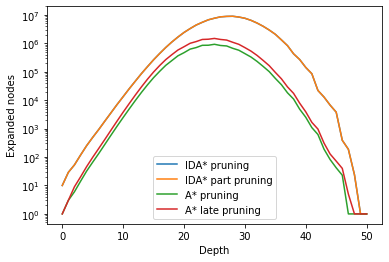
\includegraphics[scale=0.6]{15puzzle_medium.png}
      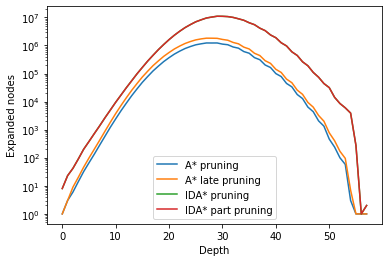
\includegraphics[scale=0.6]{15puzzle_hard.png}
      \\
      \small{\textit{Figure 1: Left, easy. Right, medium. Down, hard}}
    \end{figure*}
    
  \subsection{24 Puzzle}

  \subsection{Towers of Hanoi 4 Pegs - 12 Disks}

  \subsection{Towers of Hanoi 4 Pegs - 14 Disks}

  \subsection{Towers of Hanoi 4 Pegs - 18 Disks}

  \subsection{Top Spin 12 Tokens - Turntable of length 4}

  \subsection{Top Spin 14 Tokens - Turntable of length 4}

  \subsection{Top Spin 17 Tokens - Turntable of length 4}

  \subsection{Rubik's Cube}

\section{Detalles de Implementaci\'on}
  \subsection{NodesPriorityQueue}
    La clase \verb|NodesPriorityQueue| tiene 3 campos fundamentales:
    \begin{itemize}
      \item \verb|map<uint64_t, pair<unsigned, Node*>> hash| es un diccionario
      que mapea las valores de la tabla hash proporcionada por la API de PSVN
      a pares \verb|{V, N}| donde \verb|V| es el valor del nodo al que apunta
      \verb|N|.

      \item \verb|set<pair<unsigned, Node*>> ordered_nodes| es un conjunto de 
      pares \verb|{V, N}| con la misma definici\'on anterior. Cabe destacar 
      que el tipo de dato \verb|set| est\'a implementado en C++ como un arbol 
      rojo-negor, por lo que mantendr\'a ordenados los nodos seg\'un su valor 
      \verb|V|.

      \item \verb|unsigned (*f) (Node*)| es la funci\'on de evaluaci\'on de 
      los nodos.
    \end{itemize}

    As\'i, para buscar un nodo seg\'un su hash, simplemente tenemos que verificar
    que se encuentra en el campo \verb|hash|, lo cual es $O(1)$. Mientras que 
    para realizar el reemplazo, primero obtenemos el hash del estado que tiene 
    el nodo, luego, usando \verb|hash| obtenemos el par \verb|{V, N}|, y con ese 
    par, obtenemos el elemento que se encuentra en \verb|ordered_nodes|, y as\'i 
    realizamos el cambio en ambas estructuras en $O(\log n)$.

  
  \subsection{InformedSearchs}
    Para imprimir la memoria virtual usada actualmente se utiliza la estructura 
    \verb|struct sysinfo|, el cual, luego de aplicarle la funci\'on \verb|sysinfo|,
    almacena la memoria RAM y swap usada. As\'i, solo debemos imprimir la memoria 
    virtual inicial antes de correr el algoritmo y la memoria virtual justo antes 
    de terminar para saber aproximadamente cuanta memoria se us\'o. Para imprimir 
    el tiempo transcurrido se us\'o la funci\'on \verb|clock()|, marcando el tiempo 
    inicial e imprimiendo su diferencia con el tiempo final. \\

    Las funciones auxiliares \verb|apply_rule| y \verb|revert_rule| pueden parecer
    redundantes ya que la API de PSVN contiene las funciones \verb|apply_fwd_rule|
    y \verb|apply_bwd_rule| respectivamente. Sin embargo, estas dos \'ultimas tienen
    un problema cuando el estado al que se le aplicar\'a la regla y el estado que 
    almacenar\'a el sucesor son el mismo, probablemente porque es modificado mientras 
    es leido por la funci\'on. Es por esto que las funciones \verb|apply_rule| y 
    \verb|revert_rule| lo que hacen es generar un estado auxiliar copiando al estado 
    original, y lo usa como estado al que se le aplicar\'a la regla y almacena al 
    sucesor en el estado original. Estas son usadas por IDA* con eliminaci\'on parcial 
    de duplicados. \\

    La estructura \verb|NodesPriorityQueue| se us\'o en A* con eliminaci\'on de 
    duplicados, y realiza las funciones de almacenar los nodos ordenados seg\'un su 
    valor (costo del camino parcial m\'as la heur\'istica), y permite verificar la 
    existencia de un estado y la sustituci\'on de nodos con el mismo estado de forma 
    eficiente. \\

    Mientras que para A* con eliminaci\'on tard\'ia de duplicados se us\'o una tabla
    de hash que mapea los valores de hash para los estados dado por la API de PSVN 
    a costos parciales. As\'i, podemos verificar la existencia de un estado y su costo 
    almacenado de forma eficiente. \\ 

    Para IDA* con eliminaci\'on de duplicados se utiliz\'o una variable de tipo 
    \verb|set| que almacenaba los nodos que se encontraban en el camino actual. As\'i,
    solo basta con verificar si un nodo sucesor pertenece a dicho camino para saber 
    si se debe agregar o no.

  \subsection{PDBs}
    El proceso de generaci\'on de un PDB para un puzzle sigue los siguientes pasos:
    \begin{enumerate}
      \item Compilar el archivo \verb|abstractor.cpp| y \verb|psvn.cpp| de la API de 
      PSVN para obtener un archivo binario \verb|abstractor.out| que nos permita crear 
      la abstracci\'on que necesitamos.
      \item Utilizar \verb|abstractor.out| para generar un la abstracci\'on \verb|.psvn| 
      a partir del archivo \verb|.psvn| original y el archivo \verb|abstraction|.
      \item Ejecutar \verb|psvn2c| sobre el archivo \verb|.psvn| abstraido para generar 
      un archivo \verb|.c| que contiene las reglas del puzzle abstraido codificadas.
      \item Compilar el archivo \verb|dist.cpp| proporcionado por la API de PSVN junto 
      al \verb|.c| del paso anterior para generar un ejecutable \verb|.dist|.
      \item Ejecutar el archivo \verb|.dist|, el cual generar\'a un PDB codificado en 
      un archivo tal que cada l\'inea sigue el formato \verb|<VALUE> <STATE>|, donde 
      \verb|<VALUE>| es el costo m\'inimo desde el estado \verb|<STATE>| hacia el estado 
      objetivo. Este output es almacenado en un archivo \verb|.pdb| que puede llegar a 
      ser muy pesado.
      \item Eliminar el archivo \verb|.c| y \verb|.psvn| abstraido y luego copiar y 
      pegar el \verb|.psvn| original en el directorio actual. La raz\'on de hacer esto 
      es que para compilar el siguiente archivo necesitamos usar el psvn con las reglas 
      y estados originales.
      \item Compilar el archivo \verb|make_state_map| creado por nosotros el cual 
      inicializa una variable del tipo \verb|state_map_t| proporcionado por la API, y 
      por cada l\'inea del archivo \verb|.pdb| almacena en dicha variable el estado y 
      su valor. Luego de recorrer todo el archivo, almacena la variable de 
      \verb|state_map_t| en un archivo \verb|.state_map|.
      \item Ejecutamos \verb|make clean| para quedarnos \'unicamente con el archivo 
      \verb|.state_map|.
    \end{enumerate}

  \subsection{heuristics}
    Para evitar crear una funci\'on heur\'istica por cada puzzle del mismo tipo pero 
    con diferentes dimensiones, por ejemplo 3 funciones para Top Spin con 12, 14 y 17 
    tokens respectivamente, donde cada funci\'on ser\'a casi exactamente igual pero 
    cambiando el valor de algunas variables, decidimos utilizar variables globales 
    que definan el comportamiento de las heur\'isticas:

    \begin{itemize}
      \item \verb|vector<state_map_t*> pdbs| almacena los PDBs que se usar\'an en las 
      heur\'isticas. La funci\'on \verb|init_pdbs| permite cargar todos en \verb|pdbs|
      los archivos \verb|.state_map| que se encuentren en un directorio dado como 
      argumento. Los \verb|.state_map| son cargados en orden alfab\'etico. 

      \item \verb|unsigned (*f) (unsigned, unsigned)| es una funci\'on que indica la 
      relaci\'on entre heur\'isticas de bloques PDB, puede tomar el valor de 
      \verb|max_h| para agarrar el m\'aximo en caso de heur\'isitcas no aditivas, o 
      \verb|sum_h| para sumarlas en caso de heur\'isitcas aditivas. Las funciones que 
      realizan la asignaci\'on de \verb|f| son \verb|set_max| y \verb|set_sum|.

      \item Cada puzzle tiene su propia variable global \verb|partition| (pudiendo 
      ser de distinto tipo entre cada puzzle) que almacena la forma en que se 
      particionar\'a el puzzle para los PDBs. Es importante que el orden en el que 
      se encuentran los bloques de la partici\'on corresponda al orden en el que son 
      cargados los PDBs en la variable \verb|pdbs|, en caso contrario se obtendr\'a
      un bello y hermoso \verb|segmentation fault|. Por cada variante de un puzzle 
      existe una partici\'on correspondiente y una funci\'on que realiza la 
      asignaci\'on de la variable \verb|partition| global del puzzle gen\'erico a 
      la variable \verb|partition| del puzzle con dimensiones espec\'ificas. Por 
      ejemplo, para los NPuzzles existe una variable \verb|string **partition_Npuzzle|
      y para el 15Puzzle y 24Puzzle est\'an las variables 
      \verb|string partition_15puzzle[4][4]| y \verb|string partition_24puzzle[5][5]|
      junto a las funciones \verb|set_15puzzle| y \verb|set_24puzzle| respectivamente 
      que asignan a \verb|partition_Npuzzle| la partici\'on que corresponda.
    \end{itemize}

    Adem\'as, cada puzzle tiene su propia funci\'on \verb|make_state_abs| que toma un 
    estado y un bloque de la partici\'on y genera un nuevo estado abstraido seg\'un 
    dicho bloque. Una vez con estos elementos, las heur\'isticas de cada puzzle siguen 
    el mismo comportamiento: Reciben un esto, recorren el vector \verb|pdbs| y por cada 
    uno generamos un estado abstraido dado el bloque de la partici\'on correspondiente, 
    obtenemos el valor de dicho estado seg\'un el \verb|state_map| y actualizamos el 
    valor de la heur\'isitca seg\'un \verb|f|. 
\section{Conclusi\'on}

\end{document}